\documentclass{article}%
\usepackage[T1]{fontenc}%
\usepackage[utf8]{inputenc}%
\usepackage{lmodern}%
\usepackage{textcomp}%
\usepackage{lastpage}%
\usepackage[head=40pt,margin=0.5in,bottom=0.6in]{geometry}%
\usepackage{graphicx}%
%
\title{\textbf{"Arrow" terminará con su octava temporada}}%
\author{DPA}%
\date{07/03/2019}%
%
\begin{document}%
\normalsize%
\maketitle%
\textbf{URL: }%
http://www.eluniversal.com/entretenimiento/34992/arrow{-}terminara{-}con{-}su{-}octava{-}temporada\newline%
%
\textbf{Periodico: }%
EU, %
ID: %
34992, %
Seccion: %
entretenimiento\newline%
%
\textbf{Palabras Claves: }%
NO\_TIENE\newline%
%
\textbf{Derecho: }%
2.1%
, Otros Derechos: %
\newline%
%
\textbf{\textit{"The Flash", "Supergirl", "Legends of Tomorrow", "Black Lightning" y ahora "Batwoman", continuarán el legado del superhéroe de DC}}%
\newline%
\newline%
%
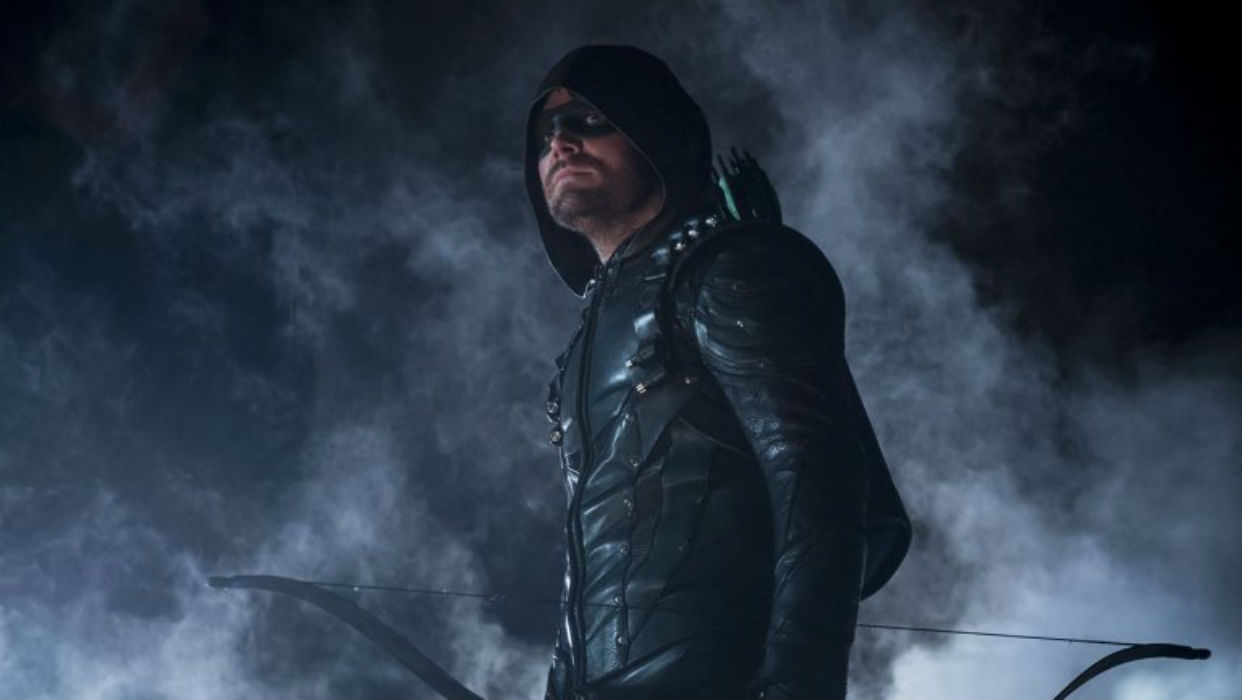
\includegraphics[width=300px]{EU_34992.jpg}%
\newline%
%
, la primera serie del Universo televisivo de DC que llegó a The CW, se despedirá con su octava temporada. La última entrega de la ficción protagonizada por Stephen Amell solo tendrá diez episodios y se estrenará este otoño.%
\newline%
%
En un comunicado que recoge The Hollywood Reporter, la showrunner de la serie, Beth Schwartz, y los productores ejecutivos Greg Berlanti y Marc Guggenheim afirman que "fue una decisión difícil de tomar, pero como todas las decisiones difíciles que tomamos en los últimos siete años, fue pensando en lo mejor para Arrow".%
\newline%
%
"Estamos felices de que Arrow creara un universo completo de espectáculos que seguirán durante muchos años", continua la declaración, "estamos entusiasmados de crear un final que honre a la serie, a sus personajes y a su legado".%
\newline%
%
Los productores también mostraron su agradecimiento a todo el equipo y a los fans que "nos han sostenido a nosotros y a la serie durante siete años".%
\newline%
%
Tras el anuncio del fin de la serie, Stephen Amell, quien dio vida al arquero desde 2012, afirmó en Twitter que "interpretar a Oliver Queen ha sido la experiencia más increíble de mi vida, pero no puedes ser un vigilante para siempre".%
\newline%
%
"Hay mucho que decir, pero por ahora les daré las gracias", concluyó.%
\newline%
%
En la gira de prensa de la Asociación de Críticos de Televisión celebrada en Pasadena (California), el presidente de la cadena, Mark Pedowitz, anunció: "Las cosas envejecen y queremos que la próxima generación de series mantenga el universo de DC en The CW el mayor tiempo posible".%
\newline%
%
La cadena ya se prepara para la próxima generación de DC. Berlanti, productor ejecutivo de todas la series de DC, se ha asociado con la showrunner Caroline Dries para la serie de Batwoman, liderada por Ruby Rose.~Su capítulo piloto está actualmente en proceso de producción.%
\newline%
%
The CW ha renovado diez de sus series en prime time para la temporada 2019{-}2020, incluidas sus cinco ficciones de superhéroes de DC que son: la octava temporada de Arrow, la quinta de Supergirl y Legends of Tomorrow, la sexta entrega para The Flash y la tercera para Black Lightning.%
\newline%
%
También estarán de vuelta Riverdale, Dinastía, Embrujadas, Sobrenatural y Legacies. Por el momento no se han revelado las fechas de estreno.%
\newline%
%
\end{document}